\ifx\ucebnice\undefined
\documentclass[a5paper,10pt,twoside]{book}
\usepackage{luatex85}
\usepackage{latexsym}
\usepackage{amsmath}
\usepackage{amsfonts}
\usepackage{amsthm}
\usepackage{amssymb}
\usepackage{fncylab}
\usepackage{comment}
\usepackage{float}
\usepackage{wrapfig}
\usepackage{tikz}
\usepackage{tikz-qtree}
\usepackage{url}
\usepackage{xcolor}
\usepackage{pdfpages}
\usepackage[czech]{babel}
\definecolor{svlinks}{rgb}{.0,0.3,0.6} %tmavě modrá
\usepackage[bookmarks, colorlinks=false,pdfhighlight=/O,linkcolor=svlinks,urlcolor=svlinks,
            pdftitle={Úvod do programování (část II: Algoritmy},
            pdfauthor={Jonathan L. Verner},
            pdfsubject={Algoritmy a složitost},
            pdfkeywords={algoritmus, složitost, Python, třídění, grafy},
            bookmarksdepth=3
            ]{hyperref}
\usepackage[toc,xindy,nopostdot,nonumberlist]{glossaries}
\usepackage[top=2cm,bottom=2cm,left=2cm,right=1cm]{geometry}
\usepackage{fancyhdr}
\usetikzlibrary{decorations.fractals,chains,fit,shapes,patterns}
% \usepackage[utf8]{inputenc}
% \usepackage[T1]{fontenc}
% \usepackage{palatino}
\usepackage{unicode-math}
\usepackage{fontspec}
\usepackage{attachfile}
\usepackage{minted}
\usepackage{multicol}
\usepackage{caption}
\usepackage{titlesec,titletoc}
\usepackage[letterspace=150]{microtype}
\relpenalty=9999
\binoppenalty=9999


% \ifblackandwhite
%   \newcommand{\logoUK}{\includegraphics[width=20mm]{UK-logo}}
%   \definecolor{UKRed}{RGB}{0,0,0}
%   \definecolor{Gray}{RGB}{0,0,0}
% \else
  \newcommand{\logoUK}{\includegraphics[width=20mm]{UK-logo-red}}
  \definecolor{UKRed}{RGB}{210,45,64}
  \definecolor{Gray}{HTML}{5e6a71}
% \fi

%----------definitions---------------------------


%math definitions

\newcommand{\R}{\mathbb R}
% \newcommand{\C}{{\mathcal C}}
\newcommand{\F}{{{\mathcal F}}}
% \newcommand{\U}{{{\mathcal U}}}
\newcommand{\V}{{{\mathcal V}}}
\newcommand{\cont}{{\mathfrak{c}}}
\newcommand{\force}{\Vdash}
\newcommand{\pw}{{{\mathcal P}}}
\newcommand{\MU}{{\mathbb{M}_{\mathcal{U}}}}
\newcommand{\pomega}{\pw(\omega)}


\newcommand{\src}[3][]{%
\begin{program}%
\caption{#3\hfill%
\attachfile[author={Jonathan Verner},
            description={Source code for #3},
            mimetype={text/x-python},
            print=false,
            color=1 1 1,
            icon={Tag}]{kod/#2.py}}
\label{alg:#2}{\inputminted[linenos]{python}{kod/#2.py}}
\end{program}}


\newcommand{\srcsplit}[4][]{%
\begin{program}%
\caption{#3\hfill%
\attachfile[author={Jonathan Verner},
            description={Source code for #3},
            mimetype={text/x-python},
            print=false,
            color=1 1 1,
            icon={Tag}]{kod/#2.py}}
\label{alg:#2}{\inputminted[linenos,lastline=#4]{python}{kod/#2.py}}
\end{program}
\begin{program}%
\caption*{#3\hfill%
(pokračování algoritmu \ref{alg:#2})}
\inputminted[linenos,firstline=#4]{python}{kod/#2.py}
\end{program}
}

\newcommand{\sniphere}[1]{%
\label{alg:#1}\inputminted[linenos]{python}{kod/#1.py}
}

\newcommand{\srchere}[3][]{%
\begin{programhere}%
\caption{#3\hfill%
\attachfile[author={Jonathan Verner},
            description={Source code for #3},
            mimetype={text/x-python},
            print=false,
            color=1 1 1,
            icon={Tag}]{kod/#2.py}}
\label{alg:#2}\inputminted[linenos,#1]{python}{kod/#2.py}
\end{programhere}}


\newcommand{\varsrc}[3][]{%
\begin{program}%
\caption{#3\hfill%
\attachfile[author={Jonathan Verner},
            description={Source code for #3},
            mimetype={text/x-python},
            print=false,
            icon={Paperclip}]{kod/#2.py}}
\label{alg:#2}\inputminted[linenos]{python}{kod/#2.py}
\end{program}}



 %% ALGORITHMS
 \floatstyle{ruled}
 \newfloat{program}{htbp}{listings}[chapter]
 \newfloat{programhere}{H}{listings}[chapter]
 \floatname{program}{Algoritmus}
 \floatname{programhere}{Algoritmus}

 % Make program and programhere share counters
% (LaTeX constructs a counter by prepending the float-name with c@
 \makeatletter
 \let\c@programhere\c@program
 \makeatother

 %---------numbering of the theorems------------
 \swapnumbers

 \newtheorem*{theorem*}{Věta}
 \newtheorem{theorem}[program]{Věta}
 \newtheorem{example}[program]{Příklad}
 \theoremstyle{definition}
 \newtheorem{definition}[program]{Definice}
 \newtheorem{question}[program]{Problém}
 \newtheorem{uloha}[program]{Úloha}
 \newtheorem{cviceni}[program]{Cvičení}
 \newtheorem{cviceniH}[program]{Cvičení (*)}
 \newtheorem*{reseniIMPL*}{Řešení}
 \specialcomment{reseni}{\begin{reseniIMPL*}}{\end{reseniIMPL*}}
 \excludecomment{reseni}
 \excludecomment{todo}
 \newtheorem*{comments*}{Komentáře}
 \newtheorem*{definition*}{Definice}
 \newtheorem{remark}[program]{Poznámka}
 \newtheorem*{note}{Poznámka}


% GLOSSARIES

\newglossary{person}{gls}{glo}{Lidé}
\DeclareRobustCommand{\textemph}[1]{\emph{#1}}
\renewcommand{\glsdisplay}[4]{\textemph{#1 (\glsentryuseri{\glslabel})}}
\newcommand{\person}[2][]{\gls{person:#2}}
\newenvironment{doplneni}{%
\par
\leftskip1cm
\rightskip1cm
\small
}{\par}

\newenvironment{python}{%
 \VerbatimEnvironment
 \begin{minted}[linenos]{python}}
{%
\end{minted}%
}

\loadglsentries[person]{people.tex}
\makeglossaries
% \printglossary[type=person,title={Lidé}]

 \hypersetup{
    colorlinks,%
    citecolor=black,%
    filecolor=black,%
    linkcolor=black,%
    urlcolor=black
}

% \pdfinfo{
%       /Author (Jonathan Verner)
%       /Title (ALG110006 Úvod do programování: Poznámky k přednášce, LS)
%       /Subject (programování, algoritmy)
%       /Keywords (quicksort,heapsort,dijsktra,graph,euclid)
%    }



% Chater & Section title formatting (uses the titlesec package)
\titleformat{\chapter}[block]{\sf\Huge\raggedright}{\hskip-1cm{\color{UKRed}\thechapter\hskip5mm\vrule}}{1em}{}
\titleformat{\section}[block]{\sf\Large}{\hskip-1cm{\color{UKRed}\thesection}}{3.5mm}{}

% Table of contents formatting
\titlecontents{chapter}
[0pt]
{\addvspace{1pc}}
{\contentsmargin{0pt}%
\makebox[0pt][r]{\sf\color{UKRed}\large\thecontentslabel\enspace}%
\sf\large}
{\contentsmargin{0pt}%
\large}
{\hfill\quad\sf\thecontentspage}
[\addvspace{2mm}]

\titlecontents{section}
[7mm]
{}
{\contentsmargin{10pt}%
\makebox[0pt][r]{\sf\color{UKRed}\thecontentslabel\enspace}%
\sf}
{\contentsmargin{10pt}}
{\hfill\quad\sf\thecontentspage}
[]



% Table of contents has two-column layout with a 2cm gap
% Note that the following can lead to conflicts with some packages
% which aggressively want to execute code AtEnd and AtBegin
% \columnsep=2cm
% \AtBeginDocument{\addtocontents{toc}{\protect\begin{multicols*}{2}}}
% \AtEndDocument{\addtocontents{toc}{\protect\end{multicols*}}}



\setsansfont{gill-sans-mt}
\setmainfont[Ligatures={Common,Rare,Historic,TeX}]{Caladea}
\setmathfont{cambria-math}
\setmonofont{Inconsolata}
\newfontfamily\Bodoni{Libre Bodoni}

%-------------opening--------------------------
\begin{document}
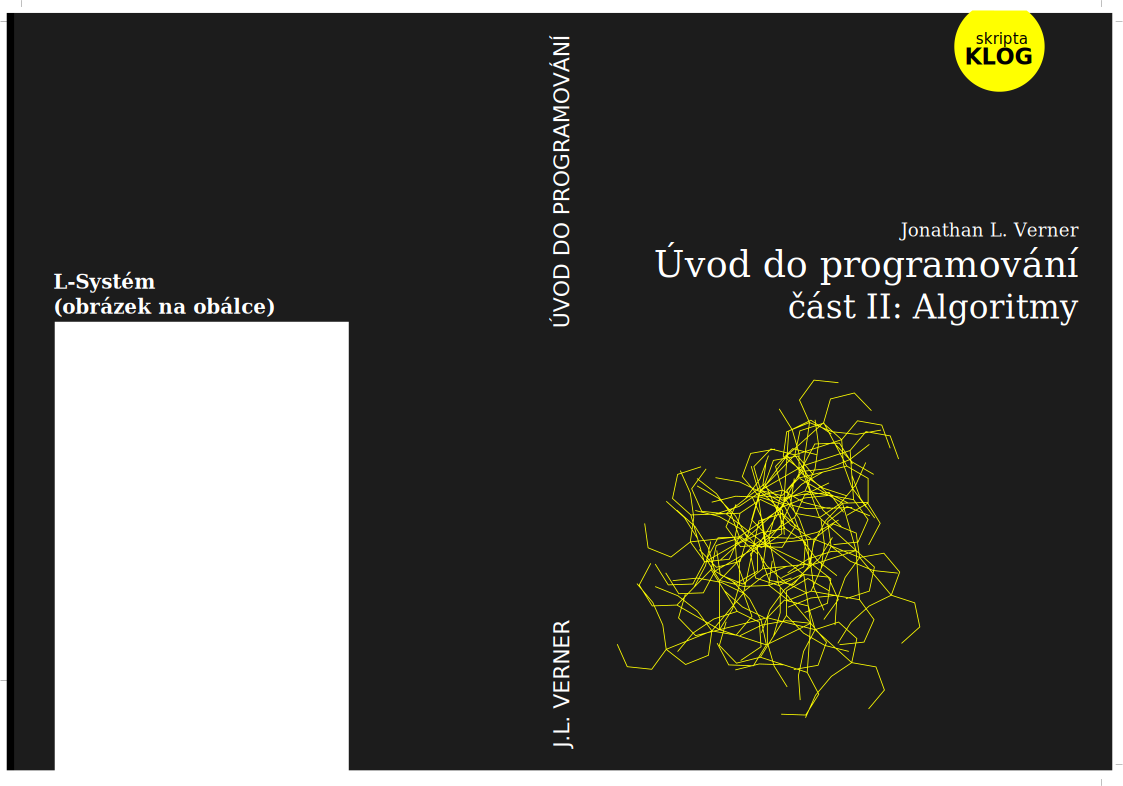
\includepdf[pages={1},noautoscale=true,fitpaper=true,offset=-8cm 0]{obalka-black.pdf}


\title{}

% \author{Jonathan Verner}
% \address{Department of Logic, Charles University\\
% Palachovo nám. 2\\ 116 38 Praha 1, Czech Republic}
% \email{jonathan.verner{@}ff.cuni.cz}
%\thanks{The author was partially supported by }

%\subjclass[2010]{Primary }
%\keywords{}

%\begin{abstract}
%\end{abstract}
%\maketitle
% \pagestyle{empty}

\headheight=12.4pt
\pagestyle{fancy}

%\hsize=16cm
\parindent=0cm
\parskip=0.2cm
\thispagestyle{empty}
\
\vskip1cm
Jonathan L. Verner, PhD.\\
Katedra Logiky\\
Filozofická fakulta UK\\
Palachovo náměstí 2\\
116 18 Praha 1
\vfill
\copyright\ Jonathan L. Verner, 2015 \\[3mm]
{\small Tato učebnice slouží jako skripta k letnímu semestru přednášky
\emph{Úvod do programování}, vypsané pod kódem ALG110006 na Katedře logiky FF UK
v letech 2011--2015. Jejich příprava byla podpořena projektem
OPVK CZ.1.07/2.2.00/28.0216 \emph{Logika: systémový rámec rozvoje oboru v ČR a
koncepce logických propedeutik pro mezioborová studia}\\}


\includegraphics[width=12cm]{logolink}
\eject
\thispagestyle{empty}
\
\vskip3cm
\begin{center}
 \sf\Huge Úvod do programování\\[1cm]
 \sf\Large část II: Algoritmy
\end{center}
\vfill
\eject

\lhead[\sf{\bf\thepage}]{\sf\nouppercase{\leftmark}}
\rhead[\sf\nouppercase{\leftmark}]{\sf\bf\thepage}
\cfoot{}

\tableofcontents

\setcounter{section}{0}
\fi
\section{Porovnávání algoritmů, Eukleidův algoritmus}

Mým cílem v zimním semestru bylo Vás naučit psát jednoduché programy v Pythonu a mít nějakou konkrétní představu o tom,
co to prakticky znamená ``programovat''. V letním semestru se podíváme na programování z teoretičtějšího hlediska.
Naším základním tématem budou různé algoritmy --- standardní (ale i nestandardní) postupy řešení různých problémů, 
se kterými se jako programátoři můžete potkat. 

Pojďme se nyní společně podívat na jednu skupinu takových problémů. Jedná se o problémy, které původně pocházejí z
matematické disciplíny zvané Teorie čísel. V praxi jsou úzce provázány s moderními šifrovacími metodami 
(RSA, Elektronický podpis, ...). Asi nejvíce fascinujícím problémem je následující úloha:

\begin{ukol}
Nalezněte rozklad daného čísla $n$ na součin prvočísel.
\end{ukol}

s ní úzce souvisí úloha, ve které máme rozhodnout, zda číslo je, či není prvočíslem:

\begin{ukol}
Pro dané číslo $n$ rozhodněte, zda je prvočíslem nebo není.
\end{ukol}

K této úloze se možná, pokud zbyde čas, vrátíme v nějaké pozdější přednášce. Dnes se podíváme na jednodušší úlohu, která
bývá jednou ze základních operacích prováděných při řešení složitějších problémů v teorii čísel. 

\begin{ukol}
Pro dané čísla $n,m$ zjistěte jejich největšího společného dělitele.
\end{ukol}

% \begin{comments*} Předně je zřejmé, že když znám řešení první úlohy, není těžké vyřešit i zbylé dvě úlohy. Toto triviální
% pozorování není úplně od věci. Vtip s vařením vajíčka o převedení úlohy na známý případ.
% \end{comments}

Pokud bychom chtěli úlohu řešit na počítači, pravděpodobně by nás jako první napadlo prostě
projít všechna čísla od $1$ do $\min \{n,m\}$ a najít největší číslo, které dělí obě čísla najednou.
V Pythonu by takový algoritmus mohl vypadat třeba takto:

\begin{python}
def gcdN(n,m):
    ret = 1
    for d in range(2,n+1):
        if d % n == 0 and d % m == 0:
            ret = d
    return d
\end{python}

Možná, že někteří z Vás se s touto úlohou setkali na střední škole. Tam jste se mohli dozvědět o postupu, který 
popsal již \person{Euklides}: vezmeme větší z obou čísel a spočítáme si zbytek po dělení menším z obou čísel. Pokud je
zbytek 0, jsme hotovi (nsd je menší z obou čísel). V opačném případě provedeme totéž, tentokrát s menším číslem 
a spočítaným zbytkem. V Pythonu bychom tento postup mohli, pomocí rekurze, zapsat následovně:

\begin{python}
def gcdE(n,m):
    if n > m:
        n,m = m,n
    z = m % n
    if z == 0:
        return n
    return gcdE(z,n)
\end{python}

Pokud bychom se chtěli vyhnout rekurzi, mohli bychom stejný algoritmus napsat takto:

\src{gcdnre}{Eukleidův algoritmus (nerekurzivní verze)}

U tohoto algoritmu nemusí být na první pohled jasné, jak funguje. Dokonce není jasné, zda vůbec skončí a pokud ano, zda
dá správnou odpověď.  Jednou možností, jak zjistit, jestli algoritmus funguje, je vyzkoušet ho na několika vstupech a 
zkontrolovat odpovědi. To nám však nedá odpověď s naprostou jistotou.  Abychom si byli naprosto jistí, musíme
algoritmus pochopit a přesvědčit se, že opravdu funguje. O to se nyní pokusíme. 

Nejprve si ukážeme, že
algoritmus opravdu skončí.  První, rekurzivní verze algoritmu, nám dává i návod: u rekurzivních algoritmů dokážeme,
že skončí, pokud se přesvědčíme, že skončí v nějakém základním případě (případech) a všechny ostatní vstupy postupně převede
na tento základní případ(y).  U našeho algoritmu bude základním případem situace, kdy $n$ dělí $m$ (což budeme značit $n|m$).  Ukážeme, že rekurzivní volání
postupně převede každý vstup na tuto základní situaci. Označme si $n_0 = n$ a $m_0=m$ počáteční vstupy a $n_k, m_k$ hodnoty proměnných 
$d$, $n$ při $k$-tém průchodu řádkem 7 (t.j. $n_k$ a $m_k$ budou hodnoty parametrů při $k$-tém (rekurzivním) volání funkce {\tt gcdE}).

Všimněme si, že $0\leq n_{k+1} = m_k\ (\mbox{mod}\ n_k) <n_k$. Tedy posloupnost $n_k$ je zdola omezená
nulou a ostře klesá. Tudíž musí být konečná, tedy program musí skončit. Tudíž algoritmus provede řádek 7 pouze konečněkrát a tedy v konečném
čase skončí. 

Když už víme, že algoritmus skončí, musíme se ještě přesvědčit, že dá správnou odpověď.  Opět využijeme rekurzivní verzi.  Pokud algoritmus
skončí v základním případě (řádek 6), zjevně dá správnou odpověď. Pokud ještě ukážeme, že i na řádku 7 získáme správnou odpověť, t.j. že {\tt gcdE(n,m) = gcd(z,n)},
budeme hotovi. Poslední rovnost však plyne z následujících jednoduchých pozorování:

\begin{itemize}
 \item Pokud $d|n$ a $d|m$ pro nějaké $m = kn + z$, pak i $d|z$.
 \item Pokud naopak $d|n$ a $d|z$, pak $d$ dělí každé $m$ tvaru $ kn + z$.
 \item Tedy, je-li $m = kn + z$ pak každý společný dělitel čísel $n,m$ je i společným dělitelem čísel $n,z$ a obráceně.
\end{itemize}

Tím jsme odpověděli na základní otázku, kterou si při seznamování s novým algoritmem musíme položit --- zda pracuje správně. Jak jsme viděli, i v takto jednoduchém
případě jde o poměrně komplikovaný proces. Mohlo by Vás napadnout, zda by nešlo tento proces nějak automatizovat. To by se hodilo zejména ve složitějších případech,
kdy je třeba nejen zkontrolovat správnost algoritmu, ale zkontrolovat i jeho bezchybnou implementaci. Obecně je odpověď , jak si ukážeme v poslední přednášce, naneštěstí
záporná. Nicméně v některých konkrétních případech to lze. Tímto problémem se zabývá oblast informatiky zvaná formální verifikace.  My se však nyní obrátíme k dalším
otázkám, které je třeba položit. Uvedli jsme si dva algoritmy pro stejnou úlohu a je přirozené se ptát, zda jsou oba stejně ``dobré''.  Tomu se budeme věnovat v následujícím oddíle.

\subsection*{Porovnávání algoritmů} 
Proto, abychom oba výše popsané algoritmy porovnali, je třeba zvolit nějaké kritérium. Kritérií může být samozřejmě mnoho,
následující seznam zdaleka není vyčerpávající:

\begin{itemize}
 \item rychlost
 \item paměťová náročnost
 \item jednoduchost, srozumitelnost
 \item elegance
 \item energetická náročnost (opravdu !)
\end{itemize}

V našem kurzu se budeme zaměřovat na první dva body (a zejména na první bod), ačkoliv jsou situace, kdy mnohem důležitějším
kritériem může být třeba jednoduchost nebo energetická náročnost.  

Pokusíme se tedy oba algoritmy porovnat z hlediska rychlosti.  Rychle však narazíme na problém: nejjednodušším způsobem,
jak algoritmy porovnat, je měřit čas $T$ od puštění programu do jeho skončení. To má svá úskalí:

\begin{itemize}
 \item tento čas bude záviset na rychlosti daného počítače, jeho zatíženosti, operačním systému, překladači, interpretu ...
 \item je to experimentální veličina o které lze těžko matematicky něco dokazovat
\end{itemize}

Budeme tedy muset ideu trochu upravit --- abstrahovat od konkrétního počítače a konkrétní implementace. Nebudeme měřit čas, 
ale určíme si množinu základních operací (přiřazením, testování booleovské podmínky ({\tt if}), aritmetická operace) a budeme počítat 
počet operací,  které program při svém běhu vykoná. Označme si toto číslo $Op$. Je zjevné, že 
toto číslo bude záviset na vstupních datech. Pokud budeme počítat největšího společného dělitele čísel
$1235468127495138$ a $2159842611264567486$ budeme muset provést více operací než při počítání společného dělitele čísel
$14$ a $35$. Tedy $Op$ bude ve skutečnosti funkce vstupních dat.

Problém s funkcí $Op$ je ten, že mnohdy je obtížné jí vyjádřit nějakým jednoduchým vzorečkem. Často pro nás proto budou
důležité spodní a horní odhady této funkce. Zkusme nyní spočítat $Op_N$ a $Op_E$ dvou výše uvedených algoritmů. Začněme
naivním algoritmem. Ten nejprve provede jedno přiřazení na řádku 2. Dále se provede $n-1$-krát cyklus, tedy $n-1$-krát
se bude testovat podmínka na řádku 4. V části těchto případů se navíc provede přiřazení na řádce 5. Tedy máme
\begin{displaymath}
 Op_N(n,m) = 1 + (n-1) + ?
\end{displaymath}
Zbývá spočítat člen $?$, t.j. v kolika případech se provede řádek 5. Pokud jsou $n,m$ nesoudělná, neprovede se nikdy.
Dolním odhadem tedy je $0$. Pokud by se řádek 5 provedl pokaždé, pak by se provedl $n-1$-krát, což je tedy horní odhad.
Přesné číslo závisí na $n$ a $m$ a nelze je jednoduše vyjádřit. Mohli bychom se pokusit o statistickou analýzu, nicméně
neuděláme to (zájemce ji může nalézet v Tao'c P, \cite{TAOCP2}). Můžeme tedy učinit následující závěr:

\begin{displaymath}
 n = 1 + (n-1) \leq Op_N(n,m) \leq 1 + 2(n-1) = 2n - 1
\end{displaymath}


Podívejme se nyní na druhý algoritmus. Zde je situace o trochu složitější. Při každém volání funkce {\tt gcdE} dochází ke 
dvěma porovnáním (2. a 5. řádek), jedné aritmetické operaci (4. řádek) a při úplně prvním volání ještě ke dvěma přiřazením 
(3. řádek, uvědomte si, že jsou to přiřazení dvě a že se tento řádek v dalších
voláních nikdy neprovede). Označme si tedy počet volání funkce {\tt gcdE} číslem $c$. Pak můžeme psát:

\begin{displaymath}
Op_E(n,m) = 2 + 3c
\end{displaymath}

Jak spočíst číslo $c$? Opět budeme pouze odhadovat. Dolní odhad je $1$ v případě, že $n$ dělí $m$. Jednoduchý horní odhad dostaneme
z úvah, které jsme prováděli při důkazu správnosti algoritmu. Zjistili jsme, že při každém rekurzivním volání je první argument ostře 
menší než při předchozím. Funkce {\tt gcdE} se tedy zavolá nejvíce $n$-krát. Tedy máme odhad

\begin{displaymath}
 5 = 2+3\leq Op_E(n,m) \leq 2 + 3n
\end{displaymath}

Na základě horního odhadu bychom mohli usoudit, že první ``naivní'' algoritmus je ve skutečnosti dokonce lepší než ten složitější
Eukleidův. Musíme si však uvědomit, že skutečná hodnota $Op_E(n,m)$ může být (a, jak za chvíli
uvidíme, opravdu je) mnohem menší než výše uvedený odhad. K odvození lepšího horního odhadu zavedeme následující značení. Nechť
$n_k,m_k$ je hodnota parametrů při $k$-tém volání funkce {\tt gcdE}. Pak platí následující:

\begin{itemize}
 \item $m_{k+1}=n_k$
 \item $n_{k+1}\leq m_k/2$
\end{itemize}

První bod je zřejmý uvažujme nad druhým. Vyjděme z toho, že $n_{k+1} = m_k\ \mbox{mod}\ n_k$. Je-li $m_k>=2n_k$, pak $m_k/2>=n_k$, zatímco
zbytek po dělení $n_k$ je vždy $< n_k$, tedy v tomto případě bod platí. Je-li naopak $m_k \in (n_k, 2n_k)$ [uvědomme si, že $m_k > n_k]$, pak 
$m_k\ \mbox{div}\ n_k = 1$, tedy $m_k\ \mbox{mod}\ n_k = m_k-n_k$. Nyní opět jednoduše $n_{k+1} >= m_k/2$. 

Kombinací prvních dvou bodů máme

\begin{itemize}
 \item $n_{k+2}\leq n_k/2$
\end{itemize}

a opakovaným aplikováním tohoto bodu dostaneme

\begin{itemize}
 \item $n_{2k}\leq n_k/2^{k}$
\end{itemize}

Zjistili jsme tedy, že velikost prvního parametru se nejen ostře snižuje, ale dokonce se po dvou voláních sníží na polovinu původní hodnoty. Tedy
$0$ (resp. $1$) dosáhne po $2\lceil \log_2 n_0\rceil$ (jednoduchým dosazením do předchozího bodu zjistíme, že pro $c=2\lceil \log_2 n_0\rceil$ máme
$n_c\leq1$), tedy veličinu $c$ můžeme shora odhadnout pomocí tohoto výrazu. Celkově tedy dostáváme

\begin{displaymath}
 Op_E(n,m) \leq 2 + 3(2\lceil \log_2 n\rceil)\leq 5 + 6\log_2 n
\end{displaymath}

Zůstaňme ještě chvíli u hodnot veličiny $Op$. Tato veličina byla zavedená tak, aby dostatečně abstrahovala od času, který bude program běžet. 
Na druhou stranu od ní stále intuitivně očekáváme, že bude s tímto časem nějak blízce souviset. Tato souvislost bude samozřejmě záviset na
zvolených ``základních operacích'', programovacím jazyce a rychlosti počítače. Obecně však není nerozumné předpokládat, že tento vztah bude
``zhruba lineární'', t.j. pro každou konkrétní situaci budou existovat nějaké konstanty $K,k$ (vyjadřující např. rychlost počítače a podobné okolnosti) takové, 
že vztah mezi $Op$ a $T$ půjde vyjádřit pomocí nerovností

\begin{displaymath}
 T/K - k \leq Op \leq KT - k
\end{displaymath}

Protože veličiny $T$ a $Op$ typicky závisí na vstupních datech (t.j. jsou funkcemi nějaké proměnné $n$) a pro malá $n$ je tato nerovnost často
nezajímavá, budeme se zajímat o limitní formu této nerovnosti. Zaveďme nyní následující značení. Jsou-li $f,g$ funkce proměnné $n$ budeme psát

\begin{displaymath}
 f(n) = O(g(n)) \iff (\exists K,n_0)(\forall n>n_0)(f(n)\leq Kg(n))
\end{displaymath}

a

\begin{displaymath}
 f(n) = \Omega(g(n)) \iff (\exists K,n_0)(\forall n>n_0)(g(n)/K\leq f(n))
\end{displaymath}

První definice říká, že pro dostatečně velká $n$ je funkce $f$ shora omezená funkcí $g$ až na nějakou multiplikativní konstantu. Podobně
druhá definice říká, že je tato funkce omezená zdola až na multiplikativní konstantu. O nějakém algoritmu $A$ pracujícím s daty reprezentovanými
proměnnou $n$ řekneme, že má složitost $O(g(n))$, pokud $Op_A(n) = O(g(n))$ \emph{a zároveň} $Op_A(n) = \Omega(g(n))$. Všimněme si, že v takovém
případě bude i $T_A(n) = O(g(n))$ a $T_A(n)=\Omega(g(n))$, tedy funkce $g$ v takovém případě věrně popisuje reálné chování algoritmu. Funkce $g$,
se kterými se setkáme nejčastěji, jsou následující: $1, n, \log_2 n, n, n\log_2 n, n^2, 2^n$. Těmto funkcím odpovídá i klasifikace algoritmů na
algoritmy v konstantním čase ($O(1)$), algoritmy logaritmické ($O(\log_2 n)$), algoritmy lineární ($O(n)$), algoritmy kvadratické ($O(n^2)$) resp.
polynomiální ($O(P(n))$, kde $P$ je nějaký polynom) a algoritmy exponenciální $O(2^n)$. Algoritmy, které mají nejvýše polynomiální složitost, se
obecně považují za efektivní (záleží samozřejmě na konkrétních okolnostech), zatímco algoritmy exponenciální jsou vesměs nepoužitelné (uvědomme si,
že pokud exponenciální algoritmus na některém počítači dokáže zpracovat data nejvýše velikosti $n$, na dvakrát rychlejším počítači spočítá data
pouze o jedna vyšší velikosti $n+1$).

Když jsme nyní zavedli klasifikaci algoritmů vidíme, že Eukleidův algoritmus má logaritmickou složitost, zatímco naivní algoritmus má složitost
lineární.

\ifx\ucebnice\undefined
\renewcommand{\refname}{\textbf{Literatura}}
\bibliographystyle{mujstyl}
\bibliography{ref}
\renewcommand{\glossarypreamble}{Biografické údaje jsou převzaté z \href{http://www.wikipedia.org}{Wikipedie}.}
\printglossary[type=person,title={Lidé}]
\end{document}
\fi